\section{Set Operators, Text \& Conditional Functions}

\cm{UNION}{Samenstelling}
\cm{INTERSECT}{Doorsnede}
\cm{EXCEPT}{Verschil}

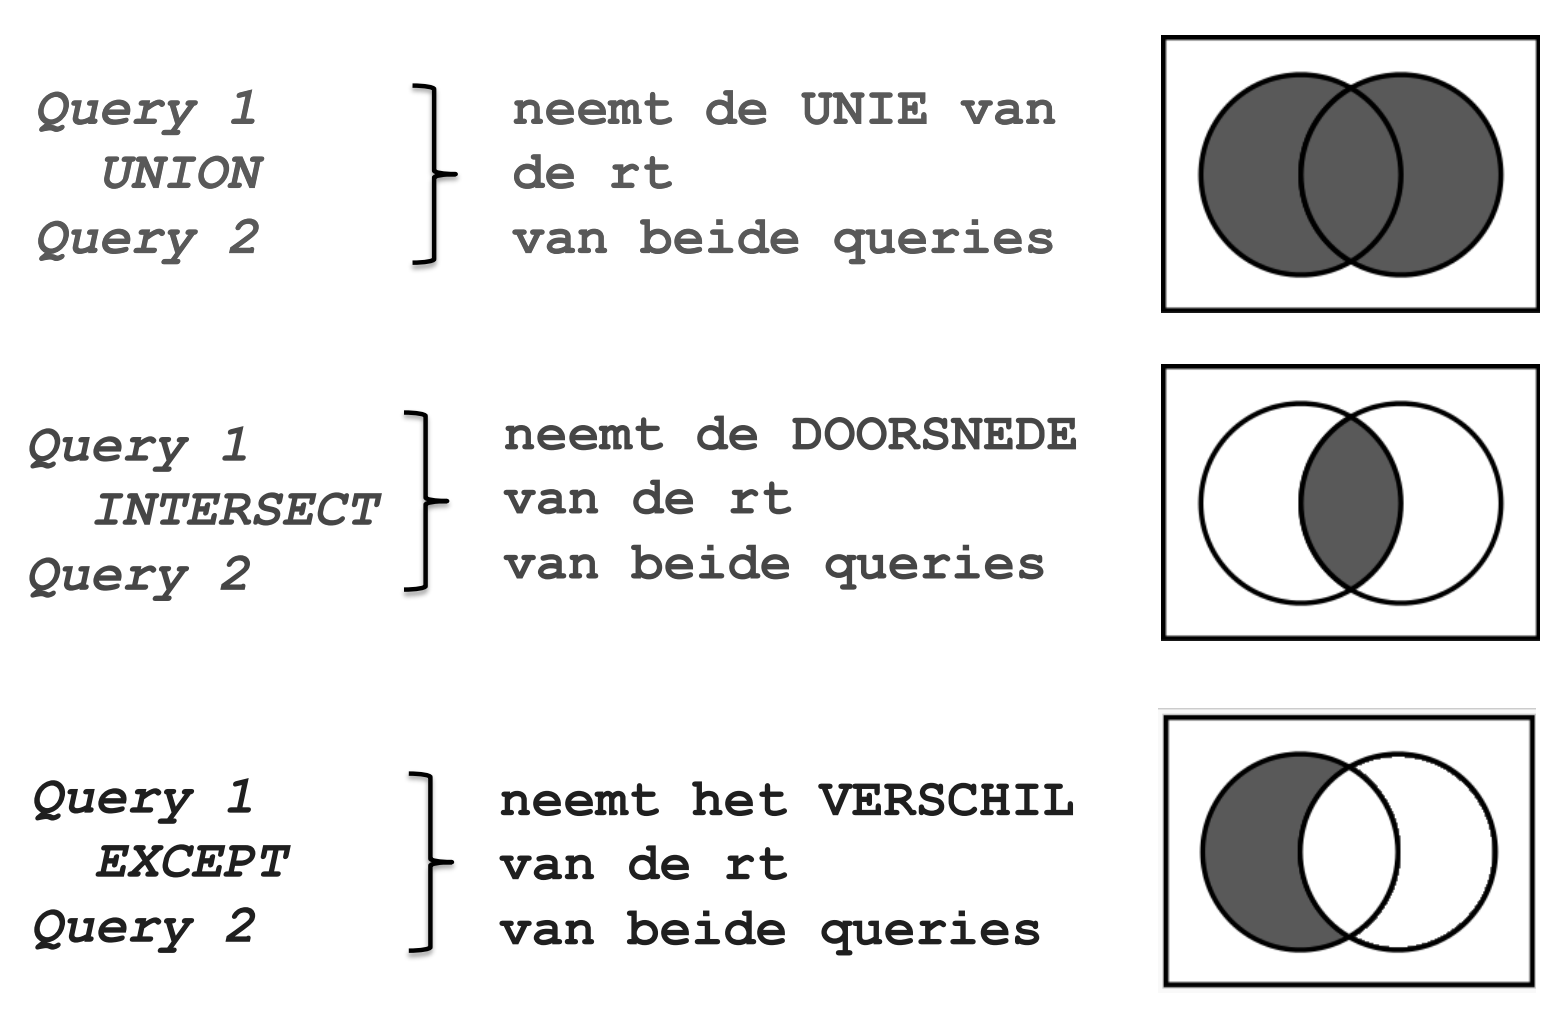
\includegraphics[scale=0.30]{./set-operatoren.png}

\subsection{UNION}
• Plaatst de rijen uit de resultatentabel van de \\
query's samen in één resultatentabel.\\
• Haalt er afhankelijk van het al dan niet aanwezig\\
zijn van de ALL optie, de dubbele rijen tussenuit

\subsection{INTERSECT}
• Plaatst alle rijen van beiden tabellen samen in één\\
resultatentabel.\\
• Haalt er de dubbele rijen tussenuit.\\

\subsection{EXCEPT}
• Plaatst de rijen uit de resultatentabel van de 1e\\
query, die niet voorkomen in de resultatentabel\\
van de 2e query in één resultatentabel.\\
• Haalt er de dubbele rijen tussenuit.\\

\subsection{SET operators combineren}
\begin{lstlisting}
SELECT1 UNION
  (SELECT2 EXCEPT SELECT3)
\end{lstlisting}